\section{Causality and sum rules}\label{sec:4.3}

No calculation has the exact excited states of silicon, yet one number about its dynamic structure factor is known exactly at every momentum transfer: the energy-weighted integral $\int\dd\omega\,\omega\,S(\vect{q},\omega)$ equals $\pi\nd_eq^2/m_e$, fixed by the electron density alone. Another exact statement ties the real part of every response function to its imaginary part. The energy-weighted integral follows from a commutator, the link between real and imaginary parts from causality, and neither depends on the interactions, the temperature or the crystal structure. The treatment follows Refs.~\cite[Sects.~3.2--3.4]{giuliani2005quantum} and \cite[Chaps.~2 and 3]{pines1966theory}.

\subsection{Kramers--Kronig relations}

The spectral form \cref{eq:4.2-spectral} already reconstructs all of $R$ from $S$, and for a diagonal element it becomes a relation between the real and imaginary parts of $R$ itself. By the fluctuation--dissipation theorem \cref{eq:4.2-fdt}, the numerator $(1 - \ee^{-\beta\omega'})S_{aa}(\vect{q},\omega')$ is $-2\Imag R_{aa}(\vect{q},\omega')$, a real function of $\omega'$, and
\begin{equation*}
  R_{aa}(\vect{q},\omega) = -\frac{1}{\pi}\int_{-\infty}^{\infty}\dd\omega'\;\frac{\Imag R_{aa}(\vect{q},\omega')}{\omega - \omega' + \ii0^+} .
\end{equation*}
The Sokhotski--Plemelj formula \cref{eq:2.4-SP} splits the denominator into a principal value and $-\ii\pi\,\delta(\omega - \omega')$. The delta function returns $\Imag R_{aa}(\omega)$ on the right, as it must, and the principal value is the real part.
\begin{keyresult}[Kramers--Kronig relations]
For a response function analytic in the upper half plane and falling off at least as $1/|\omega|$,
\begin{equation}
  \begin{gathered}
  \Real R_{aa}(\vect{q},\omega) = \frac{1}{\pi}\operatorname{PV}\!\int_{-\infty}^{\infty}\dd\omega'\,\frac{\Imag R_{aa}(\vect{q},\omega')}{\omega' - \omega}, \\
  \Imag R_{aa}(\vect{q},\omega) = -\frac{1}{\pi}\operatorname{PV}\!\int_{-\infty}^{\infty}\dd\omega'\,\frac{\Real R_{aa}(\vect{q},\omega')}{\omega' - \omega} .
  \end{gathered}
  \label{eq:4.3-KK}
\end{equation}
The dissipative part of a response, at all frequencies, fixes its reactive part at each frequency, and conversely.
\end{keyresult}
These are \cref{eq:C.5-KK}~\cite{kronig1926theory,kramers1927diffusion}. The route through \cref{eq:4.2-spectral} yields the relation for the real part from the Lehmann form. The pair of relations needs less, just the two properties of \cref{sec:4.1}: $R$ is analytic in the upper half plane, and it falls off at large $|z|$, as $1/z^2$ for a density by \cref{eq:4.1-tail}. \Cref{app:C.5} derives them from these two properties alone, by closing the integral of $R(\omega')/(\omega' - z)$ over a large semicircle in the upper half plane (\cref{fig:4-kk}a). Since that argument refers to no eigenstates, the relations hold for a measured response, for a model such as the damped oscillator of \cref{we:4-oscillator}, and for any approximation that respects causality. \Cref{fig:4-kk}b rebuilds the real part of the oscillator response from its imaginary part alone. For an off-diagonal element the same argument applies to the analytic function $R_{ab}$, with the combination $\ii(R_{ab} - R_{ba}^*)$ of \cref{eq:4.2-fdt} in the role of the absorptive part.

\begin{figure}[tbp]
  \centering
  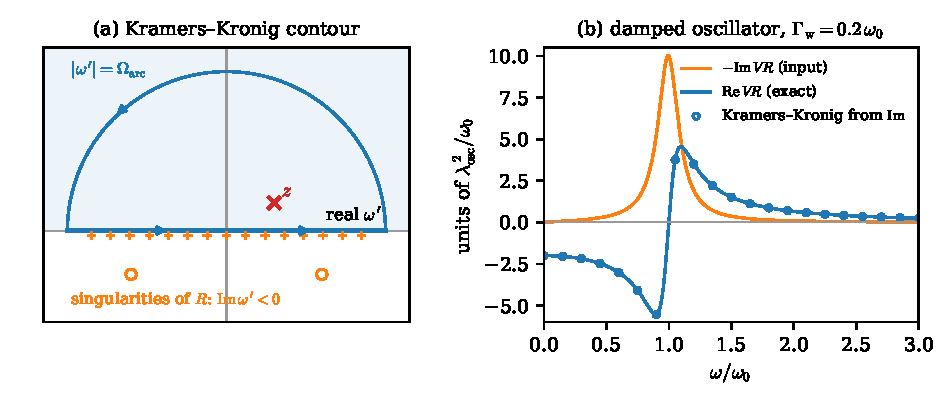
\includegraphics[width=\linewidth]{figures/ch04/fig4_3.pdf}
  \caption{The Kramers--Kronig relations. (a) The contour in the complex frequency plane $\omega'$: the real axis, closed by a semicircle of radius $\Omega_{\mathrm{arc}} \to \infty$ in the upper half plane (shaded), where the retarded response $R$ is analytic. The only singularity enclosed is the pole of $1/(\omega' - z)$ at a point $z$ of the upper half plane (cross). The singularities of $R$, the poles at transition energies that merge into a branch cut and the resonance poles of its continuation (schematic), all lie below the axis. Letting $z$ approach the real axis yields the relations. (b) Test on the damped oscillator with energy damping rate $\varGamma_{\mathrm{w}} = 0.2\,\omega_0$ and coupling $\lambda_{\mathrm{osc}}(d + d^\dagger)$. The real part of $\Vol R$ computed from $-\Imag\Vol R$ alone, with the folded relation for an even real part and an odd imaginary part (circles), agrees with the exact real part (line) to better than $10^{-11}\,\lambda_{\mathrm{osc}}^2/\omega_0$. At $\omega = 0$ both give $-2\lambda_{\mathrm{osc}}^2/\omega_0$.}
  \label{fig:4-kk}
\end{figure}

Most responses have a symmetry that folds the integral onto positive frequencies. For the density response of a target with inversion or time-reversal symmetry, the real part is even in $\omega$ and the imaginary part odd (\cref{sec:4.1}). Splitting the integral at zero and combining $1/(\omega' - \omega) + 1/(\omega' + \omega) = 2\omega'/(\omega'^2 - \omega^2)$,
\begin{equation}
  \Real R_{ee}(\vect{q},\omega) = \frac{2}{\pi}\operatorname{PV}\!\int_0^\infty\dd\omega'\,\frac{\omega'\,\Imag R_{ee}(\vect{q},\omega')}{\omega'^2 - \omega^2} ,
  \label{eq:4.3-KKhalf}
\end{equation}
which is \cref{eq:C.5-KKhalf}. Two limits of it carry physics. At $\omega = 0$, with $-2\Imag R_{ee} = (1 - \ee^{-\beta\omega})S$,
\begin{equation}
  R_{ee}(\vect{q},0) = -\frac{1}{\pi}\int_0^\infty\dd\omega\;\frac{(1 - \ee^{-\beta\omega})\,S(\vect{q},\omega)}{\omega} .
  \label{eq:4.3-static}
\end{equation}
The static response is an inverse moment of the structure factor, and it is negative because $S \ge 0$. At $T = 0$, inserting \cref{eq:4.2-Sab} returns the static limit of \cref{sec:4.1}, $\Vol R_{ee}(0) = -2\sum_f|\langle f|n_e(\vect{q})|0\rangle|^2/(E_f - E_0)$. Transitions at low energy dominate, since they are weighted by $1/\omega$: a target with a large gap is hard to deform. At large $\omega$, on the other hand, the denominator of \cref{eq:4.3-KKhalf} becomes $-\omega^2$, and $\Real R_{ee} \to -(2/\pi\omega^2)\int_0^\infty\dd\omega'\,\omega'\,\Imag R_{ee}$. The tail \cref{eq:4.1-tail} fixes the same coefficient by a double commutator. Equating the two, the energy-weighted integral of the absorptive part is fixed by an equal-time average. This is the first of the sum rules.

\subsection{Moments from commutators}

The $k$-th frequency moment of $S_{ab}$ weights each transition $i \to f$ with $\omega_{fi}^k$, where $\omega_{fi} = E_f - E_i$. The same power appears in a nested commutator. For any operator $X$, $\langle f|[H, X]|i\rangle = \omega_{fi}\langle f|X|i\rangle$, and $k$ commutators with $H$ give $\omega_{fi}^k$. Take operators with $O(-\vect{q}) = O(\vect{q})^\dagger$, as for every density, and write $[H, O_b]_k$ for $O_b$ commuted $k$ times with $H$. In the average of $[O_a^\dagger, [H, O_b]_k]$ over any state diagonal in the energy basis, with weights $p_i$, we insert a complete set $|f\rangle$ between the two operators. The term $O_a^\dagger[H, O_b]_k$ contributes $\sum_{i,f}p_i\,\omega_{fi}^k\langle i|O_a^\dagger|f\rangle\langle f|O_b|i\rangle$, the $k$-th moment of $\Vol S_{ab}(\vect{q},\omega)/2\pi$ by \cref{eq:4.2-Sab}. The term $[H, O_b]_kO_a^\dagger$ contributes $\sum_{i,f}p_i\,\omega_{if}^k\langle i|O_b|f\rangle\langle f|O_a^\dagger|i\rangle$. Since $O_b = O_b(-\vect{q})^\dagger$ and $O_a^\dagger = O_a(-\vect{q})$, this is $(-1)^k$ times the $k$-th moment of $\Vol S_{ba}(-\vect{q},\omega)/2\pi$. Altogether,
\begin{equation}
  \frac{1}{\Vol}\bigl\langle[O_a(\vect{q})^\dagger, [H, O_b(\vect{q})]_k]\bigr\rangle = \int_{-\infty}^{\infty}\frac{\dd\omega}{2\pi}\;\omega^k\,\bigl[S_{ab}(\vect{q},\omega) - (-1)^kS_{ba}(-\vect{q},\omega)\bigr] .
  \label{eq:4.3-moments}
\end{equation}
Since the derivation used only the stationarity of the state, \cref{eq:4.3-moments} holds in the Gibbs state at any temperature, in any eigenstate, and with any interactions. The integral runs over negative $\omega$ too, where a thermal target gives up energy. For $k = 0$ the left side is an equal-time commutator, and for densities, which commute with one another, it vanishes. The case $k = 1$ is the one with content.
\begin{keyresult}[First-moment identity]
For operators with $O(-\vect{q}) = O(\vect{q})^\dagger$ and any stationary state,
\begin{equation}
  \mathscr{M}^1_{ab}(\vect{q}) \equiv \frac{1}{\Vol}\bigl\langle[O_a(\vect{q})^\dagger, [H, O_b(\vect{q})]]\bigr\rangle = \int_{-\infty}^{\infty}\frac{\dd\omega}{2\pi}\;\omega\,\bigl[S_{ab}(\vect{q},\omega) + S_{ba}(-\vect{q},\omega)\bigr] .
  \label{eq:4.3-firstmoment}
\end{equation}
The energy-weighted spectrum, summed over $\pm\vect{q}$, is an equal-time double commutator.
\end{keyresult}
The first-moment matrix $\mathscr{M}^1_{ab}$ is the coefficient of $1/z^2$ in the tail \cref{eq:4.1-tail}, now read as a statement about $S$. On the diagonal, for a target with $S_{aa}(-\vect{q},\omega) = S_{aa}(\vect{q},\omega)$, it reads $\int\dd\omega\,\omega\,S_{aa} = \pi\mathscr{M}^1_{aa}$. A double commutator is often far simpler than the states it sums over, and this is why the identity is useful. The oscillator of \cref{we:4-oscillator} is the smallest example: $[O, [H, O]] = 2\lambda_{\mathrm{osc}}^2\omega_0$ is a number, and the first moment of its structure factor, $2\pi\lambda_{\mathrm{osc}}^2\omega_0$, does not depend on temperature, the result found from the populations in \cref{we:2-oscillator}. \Cref{chap:8} builds the higher moments into matrices for several operators.

\subsection{The f-sum rule}

For the electron density the double commutator is a number. The Hamiltonian of electrons and nuclei of \cref{sec:2.3} is the kinetic energy of the particles plus a potential energy that depends on their positions alone, and so do any external static potentials. The density $n_e(\vect{q}) = \sum_j\ee^{\ii\vect{q}\cdot\vect{r}_j}$ commutes with every position and with every nuclear momentum. Only the electron kinetic energy is left in $[H, n_e(\vect{q})]$. For one electron, $[\vect{p}, \ee^{\ii\vect{q}\cdot\vect{r}}] = \vect{q}\,\ee^{\ii\vect{q}\cdot\vect{r}}$, and $[\vect{p}^2, \ee^{\ii\vect{q}\cdot\vect{r}}] = \vect{p}\cdot\vect{q}\,\ee^{\ii\vect{q}\cdot\vect{r}} + \ee^{\ii\vect{q}\cdot\vect{r}}\,\vect{q}\cdot\vect{p}$. Summed over electrons,
\begin{equation}
  [H, n_e(\vect{q})] = \vect{q}\cdot\vect{j}_e(\vect{q}), \qquad \vect{j}_e(\vect{q}) = \sum_j\frac12\Bigl\{\frac{\vect{p}_j}{m_e},\,\ee^{\ii\vect{q}\cdot\vect{r}_j}\Bigr\} ,
  \label{eq:4.3-continuity}
\end{equation}
exactly, with $\{A, B\} = AB + BA$. This is the continuity equation in operator form. In the Heisenberg picture $\partial_tn_e(\vect{q},t) = \ii[H, n_e(\vect{q},t)] = \ii\vect{q}\cdot\vect{j}_e(\vect{q},t)$, the transform with $\ee^{+\ii\vect{q}\cdot\vect{r}}$ of $\partial_t\op{\nd}_e(\vect{r}) + \nabla\cdot\vect{j}_e(\vect{r}) = 0$ for the density operator of \cref{sec:4.2} and the current density in position space: density at $\vect{q}$ changes only because electrons carry it away. The symmetrized $\vect{j}_e(\vect{q})$ is what the literature calls the paramagnetic current, the current of the electrons when no vector potential acts.

The outer commutator, with $n_e(\vect{q})^\dagger$, is a number. Conjugating by the plane wave shifts the momentum, $\ee^{-\ii\vect{q}\cdot\vect{r}}\vect{p}\,\ee^{\ii\vect{q}\cdot\vect{r}} = \vect{p} + \vect{q}$, so $[\ee^{-\ii\vect{q}\cdot\vect{r}}, \vect{p}] = \vect{q}\,\ee^{-\ii\vect{q}\cdot\vect{r}}$, and each electron contributes $q^2/m_e$ to $[n_e(\vect{q})^\dagger, \vect{q}\cdot\vect{j}_e(\vect{q})]$ (\cref{app:D.6}). The commutator is $N_eq^2/m_e$ in every state, and $\mathscr{M}^1_{ee} = \nd_eq^2/m_e$.
\begin{keyresult}[f-sum rule]
For electrons that move in local potentials, at any temperature and with any interactions,
\begin{equation}
  \int_{-\infty}^{\infty}\dd\omega\;\omega\,S(\vect{q},\omega) = \frac{\pi\,\nd_e\,q^2}{m_e} \qquad \bigl(S(-\vect{q},\omega) = S(\vect{q},\omega)\bigr) ,
  \label{eq:4.3-fsum}
\end{equation}
and in general the same for the average of $S$ over $\vect{q}$ and $-\vect{q}$. The energy-weighted spectrum of density fluctuations counts the electrons.
\end{keyresult}
This is \cref{eq:A.7-fsum}~\cite[Sect.~3.4]{giuliani2005quantum}. The number $\nd_e$ counts every electron, core electrons included, and the nuclei may move. The normalization is $\pi$ over the whole real line. Many-body texts write the rule per particle and over positive frequencies, and the conversion is one line. At $T = 0$, $S$ vanishes for $\omega < 0$, and dividing by $2\pi\nd_e$ leads to $\int_0^\infty\dd\omega\,\omega\,S/(2\pi\nd_e) = q^2/2m_e$: per electron, and without the factor $2\pi$ of \cref{eq:4.2-Sab}, the first moment is the free recoil energy~\cite[Chap.~2]{pines1966theory}. At $T > 0$, detailed balance $S(\vect{q},-\omega) = \ee^{-\beta\omega}S(\vect{q},\omega)$ folds the negative frequencies onto the positive ones, $\int_0^\infty\dd\omega\,\omega\,(1 - \ee^{-\beta\omega})\,S = \pi\nd_eq^2/m_e$. By the fluctuation--dissipation theorem the integrand is $-2\omega\Imag R_{ee}$, which closes the loop with the large-$\omega$ limit of \cref{eq:4.3-KKhalf}.

The rule has a direct reading at large $q$. Divided by the total weight $2\pi\nd_eS^{\mathrm{st}}(\vect{q})$ of \cref{eq:4.2-static}, it gives the mean energy deposited at $T = 0$, $q^2/[2m_eS^{\mathrm{st}}(\vect{q})]$. Where $S^{\mathrm{st}} \to 1$ and the dark matter scatters on one electron at a time, the mean energy deposited tends to the free recoil energy, however strongly the electron is bound. Binding moves the weight around, broadening it as in the impulse approximation of \cref{we:4-gas}, but it cannot shift its center. At small $q$, where $S^{\mathrm{st}}$ is suppressed, the mean energy lies far above $q^2/2m_e$, and in the interacting electron gas the plasmon carries all of the sum (\cref{sec:4.5}).

The right side of \cref{eq:4.3-fsum} defines the frequency scale of the electrons. With $e^2 = 4\pi\alpha$,
\begin{equation}
  \frac{\pi\nd_eq^2}{m_e} = \frac{\pi q^2}{e^2}\,\omega_p^2, \qquad \omega_p^2 = \frac{e^2\nd_e}{m_e} ,
  \label{eq:4.3-wp}
\end{equation}
where $\omega_p$ is the plasma frequency, the frequency at which the electrons, treated as free, would oscillate together against a uniform positive background (\cref{sec:4.5}). For the valence density of silicon, $\nd_e = \SI{2.00e23}{cm^{-3}}$, $\omega_p = \SI{16.6}{eV}$; for all 14 electrons per atom, $\SI{7.00e23}{cm^{-3}}$, it is \SI{31.1}{eV}. \Cref{sec:4.4} converts \cref{eq:4.3-fsum} into the form $\int_0^\infty\dd\omega\,\omega\,L = (\pi/2)\,\omega_p^2$ for the loss function, the form that a computed or measured spectrum is usually tested against.

\subsection{Nonlocal potentials and the f-sum rule}

The derivation of \cref{eq:4.3-fsum} needed one hypothesis: every potential energy in $H$ is a function of positions. The Hamiltonian of electrons and nuclei satisfies it, but the effective Hamiltonians with which solids are computed often do not. A pseudopotential (\cref{sec:3.5}) replaces the nucleus and the core electrons by a local potential and a nonlocal part $V_{\mathrm{NL}}$, the sum of projections \cref{eq:E.2-KB}, which acts on a valence wavefunction through its values over a whole core region rather than at one point. The Fock exchange operator is nonlocal in the same sense. Such an operator does not commute with $\ee^{\ii\vect{q}\cdot\vect{r}}$, the commutator $[H, n_e(\vect{q})]$ acquires $[V_{\mathrm{NL}}, n_e(\vect{q})]$ besides $\vect{q}\cdot\vect{j}_e$, and
\begin{equation}
  \mathscr{M}^1_{ee}(\vect{q}) = \frac{\nd_eq^2}{m_e} + \frac{1}{\Vol}\bigl\langle[n_e(\vect{q})^\dagger, [V_{\mathrm{NL}}, n_e(\vect{q})]]\bigr\rangle ,
  \label{eq:4.3-fsumNL}
\end{equation}
with $\nd_e$ now the density of the valence electrons that the calculation keeps. The exact rule is not violated, since it belongs to the full Hamiltonian. The pseudo-Hamiltonian is a device that reproduces the valence states outside the cores, not their every commutator. A pseudo-wavefunction is smooth where the true valence state oscillates to stay orthogonal to the core states, and part of what that oscillation does is carried by $V_{\mathrm{NL}}$. The extra term is a sum of projections and costs almost nothing to evaluate. \Cref{app:E.2} writes it for one electron, \cref{eq:E.2-fsumNL}, and finds that in a representative silicon calculation this term and the truncated band sum together put the computed sum 12 to 19 percent below the local value at small $q$. A sum-rule test of a pseudopotential calculation therefore compares with \cref{eq:4.3-fsumNL}, not with \cref{eq:4.3-fsum}. At $q \to 0$ the same algebra turns the momentum into the velocity $\ii[H, \vect{r}] = \vect{p}/m_e + \ii[V_{\mathrm{NL}}, \vect{r}]$, the form that Ismail-Beigi, Chang and Louie derived for the coupling of a nonlocal potential to a long-wavelength field~\cite{ismailbeigi2001coupling}.

Relativistic electrons break the hypothesis in a different way. To order $1/m_e^2$, an electron in a one-body potential $U_1(\vect{r})$ has three corrections, derived in \cref{app:C.15}: the mass--velocity term $-\vect{p}^4/8m_e^3$, the Darwin term $\nabla^2U_1/8m_e^2$ and the spin--orbit term $\vect{\sigma}\cdot(\nabla U_1\times\vect{p})/4m_e^2$. The Darwin and spin--orbit terms drop out of the double commutator, and the mass--velocity term does not (\cref{app:D.6}). In an atom, or in a crystal of cubic symmetry,
\begin{equation}
  \mathscr{M}^1_{ee}(\vect{q}) = \frac{\nd_eq^2}{m_e}\Bigl[1 - \frac53\,\frac{\bar K}{m_e} - \frac{q^2}{4m_e^2}\Bigr] ,
  \label{eq:4.3-mv}
\end{equation}
where $\bar K$ is the mean kinetic energy per electron. A moving electron is heavier, and the f-sum, which counts electrons weighted by $1/m_e$, is reduced by the relative order $\bar K/m_e$. For silicon the virial theorem makes the total kinetic energy of the atom minus its total energy, \SI{7.86}{keV} from the Hartree--Fock value of $-288.854$ hartree~\cite{bunge1993roothaan}, so $\bar K = \SI{561}{eV}$ and $(5/3)\bar K/m_e = 1.8\times10^{-3}$, or 0.026 electrons per atom. The two 1s electrons dominate: each has a kinetic energy near $Z^2\alpha^2m_e/2 = \SI{2.67}{keV}$, which reduces its own share of the sum by $8.7\times10^{-3}$. The term in $q^2$ is $2.7\times10^{-3}$ at the \SI{53}{keV} that a \SI{10}{MeV} particle can transfer at most. The two-body Breit terms, which depend on the momenta of pairs of electrons, contribute at the same relative order, and we do not estimate them. All of these corrections lie below the accuracy of any calculation of $S$ for dark matter. They do mean, however, that an all-electron relativistic calculation with positive-energy states alone should not reproduce \cref{eq:4.3-fsum} to better than a few parts in $10^3$. The expansion in $1/m_e$ is this positive-energy statement. The full Dirac Hamiltonian is linear in the momentum, its double commutator with the density vanishes, and the f-sum is then carried by the creation of electron--positron pairs, at energies near $2m_e$.

The nuclei obey the same algebra as the electrons. With the density $n_\kappa(\vect{q}) = \sum_{I\in\kappa}\ee^{\ii\vect{q}\cdot\vect{X}_I}$ of the nuclei of species $\kappa$, their mass $M_\kappa$ and number density $\nd_\kappa$ (\cref{sec:2.3}), the kinetic energy of the nuclei gives $[H, n_\kappa(\vect{q})] = \vect{q}\cdot\vect{j}_\kappa(\vect{q})$, with a current $\vect{j}_\kappa$ built like $\vect{j}_e$ from nuclear momenta and $M_\kappa$. A current of one species contains only that species' momenta, and it commutes with the density of every other species. The mixed double commutators therefore vanish.
\begin{keyresult}[Species-resolved f-sum rule]
For electrons and nuclei in local potentials, with $s, s' \in \{e, \kappa\}$ and $m_s$ equal to $m_e$ or $M_\kappa$,
\begin{equation}
  \mathscr{M}^1_{ss'}(\vect{q}) = \delta_{ss'}\,\frac{q^2\,\nd_s}{m_s} .
  \label{eq:4.3-species}
\end{equation}
Each species has its own f-sum, fixed by its density and mass, and the energy-weighted electron--nucleus interference vanishes.
\end{keyresult}
The nuclear rule, $\int\dd\omega\,\omega\,S_{\kappa\kappa} = \pi\nd_\kappa q^2/M_\kappa$, makes the mean energy deposited on a nucleus equal to its free recoil energy $q^2/2M_\kappa$ wherever $S^{\mathrm{st}}$ of the nuclei is one, the incoherent limit of the lattice response of \cref{chap:5,chap:6}. The mixed rule has a less obvious consequence. For a target with inversion symmetry, $S_{\kappa e}(-\vect{q},\omega) = S_{\kappa e}(\vect{q},\omega)$, which Hermiticity makes $S_{e\kappa}(\vect{q},\omega)^*$, and \cref{eq:4.3-firstmoment} with \cref{eq:4.3-species} reads $\int\dd\omega\,\omega\Real S_{e\kappa}(\vect{q},\omega) = 0$. At $T = 0$ the integral runs over $\omega > 0$ alone, and the real part of the electron--nucleus interference must change sign: the electrons follow a recoiling nucleus in phase at some energies and against it at others. A computed interference spectrum of one sign, for the Migdal effect for instance (\cref{chap:8}), is wrong. Finally, for the total charge density $n_Z = -n_e + \sum_\kappa Z_\kappa n_\kappa$ of \cref{sec:2.3}, the diagonal terms add: $\mathscr{M}^1_{ZZ} = q^2[\nd_e/m_e + \sum_\kappa Z_\kappa^2\nd_\kappa/M_\kappa]$. For silicon, with $Z_\kappa = 14$ and all 14 electrons per atom, the nuclear share is $14\,m_e/M_\kappa = 2.73\times10^{-4}$. A probe of the total charge, such as a dark photon, sees an f-sum set by the electrons to that accuracy.

\subsection{Oscillator strengths}

For a single atom the f-sum rule becomes a statement about its spectral lines. Take an atom with $Z$ electrons in its ground state $|0\rangle$. Its double commutator is $Zq^2/m_e$, and inserting the excited states $|n\rangle$ as in \cref{eq:4.3-moments} turns it into $\sum_n(E_n - E_0)\bigl[|\langle n|n_e(\vect{q})|0\rangle|^2 + |\langle n|n_e(-\vect{q})|0\rangle|^2\bigr]$. For a ground state with inversion symmetry the two terms are equal, and
\begin{equation}
  \sum_n(E_n - E_0)\,\bigl|\langle n|n_e(\vect{q})|0\rangle\bigr|^2 = \frac{Zq^2}{2m_e} ,
  \label{eq:4.3-atomq}
\end{equation}
at every $\vect{q}$. For the gas of atoms of \cref{we:4-hydrogen}, whose structure factor is $2\pi\nd_T$ times the sum of these transition weights, it is \cref{eq:4.3-fsum} with $\nd_e = Z\nd_T$. As $q \to 0$, the matrix element to an excited state starts at first order in $q$, $\langle n|n_e(\vect{q})|0\rangle = \ii\vect{q}\cdot\langle n|\sum_j\vect{r}_j|0\rangle$, since the zeroth order vanishes by orthogonality. The dipole matrix elements that remain define the oscillator strengths,
\begin{equation}
  f^{\mathrm{osc}}_{n0} = 2m_e\,(E_n - E_0)\,\Bigl|\langle n|\sum_j\hat{\vect{q}}\cdot\vect{r}_j|0\rangle\Bigr|^2 ,
  \label{eq:4.3-osc}
\end{equation}
and \cref{eq:4.3-atomq} divided by $q^2/2m_e$ becomes the Thomas--Reiche--Kuhn rule~\cite{thomas1925zahl,reiche1925zahl,kuhn1925gesamtstarke},
\begin{equation}
  \sum_nf^{\mathrm{osc}}_{n0} = Z ,
  \label{eq:4.3-TRK}
\end{equation}
where the sum includes the continuum, as an integral of the oscillator-strength density $\dd f^{\mathrm{osc}}/\dd\omega$ over the energy $\omega = E_n - E_0$ of the absorbed quantum. In the classical picture an atom was a set of electrons bound by springs, and $f^{\mathrm{osc}}_{n0}$ counted how many of them oscillated at the frequency of line $n$. The rule says that the lines of an atom share exactly $Z$ such classical electrons. Its use is as a check. A table of computed or measured oscillator strengths, or of photoabsorption cross-sections, must add up to $Z$, and a set of ionization form factors (\cref{eq:2.2-fion}) must satisfy \cref{eq:4.3-atomq} at each $q$, which tests the normalization of the continuum.

\begin{workedexample}{The Thomas--Reiche--Kuhn sum of hydrogen}\label{we:4-trk}
For hydrogen, $Z = 1$, and the oscillator strengths from 1s are known in closed form~\cite[Sect.~61]{bethe1957quantum}. The dipole operator reaches only p states. For the bound levels,
\begin{equation*}
  f^{\mathrm{osc}}_{np,1s} = \frac{2^8\,n^5\,(n - 1)^{2n-4}}{3\,(n + 1)^{2n+4}} ,
\end{equation*}
which is 0.4162 for 2p, and 0.0791, 0.0290 and 0.0139 for 3p to 5p. For large $n$, $[(n - 1)/(n + 1)]^{2n} \to \ee^{-4}$ and $f^{\mathrm{osc}}_{np,1s} \to (2^8/3)\,\ee^{-4}/n^3$. The levels crowd toward the binding energy $E_B = \alpha^2m_e/2 = \SI{13.6}{eV}$ of \cref{sec:2.2} with spacing $2E_B/n^3$, and their strength per unit energy tends to $(2^7/3)\,\ee^{-4}/E_B = 0.782/E_B$. The continuum takes over at the same value. With the Coulomb parameter of \cref{sec:2.2} for the ejected electron, $\xi_{\mathrm{C}} = \alpha m_e/p = [E_B/(\omega - E_B)]^{1/2}$ for $\omega > E_B$, its density is~\cite[Sect.~61]{bethe1957quantum}
\begin{equation*}
  \frac{\dd f^{\mathrm{osc}}}{\dd\omega} = \frac{2^7}{3E_B}\Bigl(\frac{E_B}{\omega}\Bigr)^4\,\frac{\exp(-4\xi_{\mathrm{C}}\operatorname{arccot}\xi_{\mathrm{C}})}{1 - \ee^{-2\pi\xi_{\mathrm{C}}}} ,
\end{equation*}
which tends to $0.782/E_B$ at threshold, where $\xi_{\mathrm{C}} \to \infty$ and $\xi_{\mathrm{C}}\operatorname{arccot}\xi_{\mathrm{C}} \to 1$.

Adding up (\cref{fig:4-trk}a), the bound levels carry 0.565, of which 2p alone carries 0.416 and the first three 0.524. The continuum carries 0.435: 0.316 within $E_B$ of the threshold, and only 0.0042 above $10E_B$, since at large $\omega$, where $\xi_{\mathrm{C}} \to 0$, the density falls as $\omega^{-7/2}$. The total is $1.000$, as \cref{eq:4.3-TRK} requires. A calculation that keeps the bound states alone fails the check by 43 percent: the continuum, which is the ionization channel of \cref{sec:2.2}, is not a correction.

The finite-$q$ rule \cref{eq:4.3-atomq} tests the same states at a dark-matter momentum transfer. At $q_0 = \alpha m_e$ its right side is exactly $q_0^2/2m_e = \alpha^2m_e/2 = E_B$. The 2p level has $|f_{1s\to2p}(q_0)|^2 = 0.061$ (\cref{we:2-hydrogen}) at the energy $\tfrac34E_B$, and contributes $0.046\,E_B$, under 5 percent of the sum, although it takes a tenth of the inelastic weight at that $q$ (\cref{we:4-hydrogen}). The rest of the energy-weighted sum lies in the continuum, at energies $\sim E_B$ and above.
\end{workedexample}

\begin{workedexample}{The f-sum of the free electron gas}\label{we:4-gasfsum}
\Cref{we:4-gas} obtained the first moment of $S^0$ from the sum over occupied states. The closed form \cref{eq:4.2-gas} must reproduce it, and integrating it shows where the weight sits. For $q > 2k_{\mathrm{F}}$, $S^0$ is the parabola between $\omega_-$ and $\omega_+$. We change variable to $x = m_e\omega/q - q/2$, which runs from $-k_{\mathrm{F}}$ to $k_{\mathrm{F}}$. Then $\omega = (q/m_e)(x + q/2)$, $\dd\omega = (q/m_e)\,\dd x$ and $S^0 = (m_e/2\pi q)(k_{\mathrm{F}}^2 - x^2)$, so that
\begin{equation*}
  \int\dd\omega\;\omega\,S^0 = \frac{q}{2\pi m_e}\int_{-k_{\mathrm{F}}}^{k_{\mathrm{F}}}\dd x\,\Bigl(x + \frac q2\Bigr)(k_{\mathrm{F}}^2 - x^2) = \frac{q}{2\pi m_e}\,\frac q2\,\frac{4k_{\mathrm{F}}^3}{3} = \frac{q^2k_{\mathrm{F}}^3}{3\pi m_e} .
\end{equation*}
The term odd in $x$, the Doppler shift from the motion of the struck electron, integrates to zero, and with $\nd_e = k_{\mathrm{F}}^3/3\pi^2$ the result is $\pi\nd_eq^2/m_e$. For $q < 2k_{\mathrm{F}}$ the linear region, $0 < \omega < \omega_1 = (q/m_e)(k_{\mathrm{F}} - q/2)$, contributes $\int\dd\omega\,\omega\,m_e^2\omega/\pi q = m_e^2\omega_1^3/3\pi q = q^2(k_{\mathrm{F}} - q/2)^3/3\pi m_e$. That is the fraction $(1 - q/2k_{\mathrm{F}})^3$ of the sum, $27/64 = 0.42$ at $q = k_{\mathrm{F}}/2$, and the parabola carries the rest. As $q \to 0$ the linear region carries the whole sum, and the mean energy $(q^2/2m_e)/S^{\mathrm{st}}$, with $S^{\mathrm{st}} \to 3q/4k_{\mathrm{F}}$, is $\tfrac23qv_{\mathrm{F}}$, which vanishes. A gapless target can place its f-sum at vanishing energies, but only because its long-wavelength fluctuations are suppressed by the Pauli hole of \cref{sec:4.2}.

A gap changes the balance. Take the valence electrons of an insulator at $T = 0$, with the nuclei clamped and the potentials local, and their share of the f-sum, collected below the core edges (\cref{we:4-sifsum}). Their inelastic $S$ vanishes below the gap $\Eg$, so $\Eg\int\dd\omega\,S \le \int\dd\omega\,\omega\,S$. By \cref{eq:4.2-static,eq:4.3-fsum}, the inelastic part of the static structure factor then obeys, to the accuracy with which the valence electrons carry their own f-sum (about 2 percent in silicon, \cref{we:4-sifsum}),
\begin{equation*}
  S^{\mathrm{st}}(\vect{q}) \le \frac{q^2}{2m_e\Eg} .
\end{equation*}
At the valence density of silicon, $k_{\mathrm{F}} = \SI{3.57}{keV}$, and with $\Eg = \SI{1.17}{eV}$ this bound lies below the free-gas value $3q/4k_{\mathrm{F}}$ for $q < 3m_e\Eg/2k_{\mathrm{F}} = \SI{0.25}{keV}$; at $q = \SI{0.1}{keV}$ it is 0.40 of it. The long-wavelength density fluctuations of an insulator vanish as $q^2$, not as $q$, and the f-sum rule is what turns the gap into this statement.
\end{workedexample}

\begin{workedexample}{The f-sum of silicon}\label{we:4-sifsum}
A silicon atom has 14 electrons, four in the valence shell and ten in the core, two 1s and eight 2s and 2p. With the full, local Hamiltonian the f-sum counts all of them, and at $q \to 0$ the Thomas--Reiche--Kuhn rule \cref{eq:4.3-TRK}, applied per atom of the crystal, gives 14. The four valence electrons absorb from the gap upward; the core electrons cannot absorb below their binding energies, which put the L edge near \SI{100}{eV} and the K edge at \SI{1.84}{keV}.

Henke, Gullikson and Davis tabulated the photoabsorption of silicon from \SI{50}{eV} to \SI{30}{keV}. Their current distribution extends down to \SI{30}{eV}, and we integrate it from there. They express it through the imaginary part $f_2(\omega)$ of the atomic scattering factor, which in the convention of the tables is $f_2 = (\pi/2)\,\omega\,\dd f^{\mathrm{osc}}/\dd\omega$ per atom~\cite{henke1993xray}. The two edges appear in the tables as steps of $f_2$, at \SI{99.8}{eV} and \SI{1.839}{keV}. Integrating $2f_2/\pi\omega$ over the regions they bound gives 0.35 between \SI{30}{eV} and the L edge, 8.46 between the L and K edges, and 1.61 above the K edge. Of the last, 0.007 comes from extending the last decade of the tables beyond \SI{30}{keV} as a power law. Above \SI{30}{eV} the tables therefore hold 10.42 of the 14. The rule then requires 3.58 below \SI{30}{eV} (3.55 with the mass--velocity reduction of \cref{eq:4.3-mv}), and 3.93 below the L edge, against the four valence electrons (\cref{fig:4-trk}b).

The saturation is slow and has the same pattern in each region. The valence part is complete to 2 percent below the L edge, at six times $\omega_p$. The region between the edges collects 97 percent of its strength by \SI{1}{keV}, ten times its edge energy, and the region above the K edge collects 84 percent by \SI{5}{keV} and 96 percent by \SI{10}{keV}. Each shell gathers its strength over energies from its edge to several times it, with the slow $\omega^{-5/2}$ approach of the remaining strength that hydrogen showed.

The regions are not the shells. The region above the K edge holds 1.61, not 2. The 1s electrons cannot be promoted into the full 2p shell, a transition that carries 0.42 of the sum in hydrogen. In a picture of independent electrons, the rule holds for each electron only when transitions into occupied orbitals are counted too, upward with positive and downward with negative strength. In the atom both members of such a pair are blocked by the Pauli principle, and since their strengths cancel, the total stays 14 while strength moves from the inner shells to the outer ones. The excess of the region between the edges over 8 is the receiving side of this transfer, together with the overlap of tails: the L absorption continues above the K edge, and the valence absorption continues above the L edge.

For dark matter the split matters at finite $q$. At $q \to 0$ the core part of the sum lies above \SI{100}{eV}, far from the valence part. At larger $q$ the valence weight moves toward the free recoil energy $q^2/2m_e$, which is \SI{98}{eV} at $q = \SI{10}{keV}$, where the dark matter can deposit at most $qv_{\mathrm{max}} = \SI{26.5}{eV}$. A valence-only calculation tested against its f-sum at such momentum transfers must follow the valence spectrum to energies where the core shells it omits absorb as well. The sum rule constrains the total over all energies, not the low-energy corner that the dark matter samples.
\end{workedexample}

\begin{figure}[tbp]
  \centering
  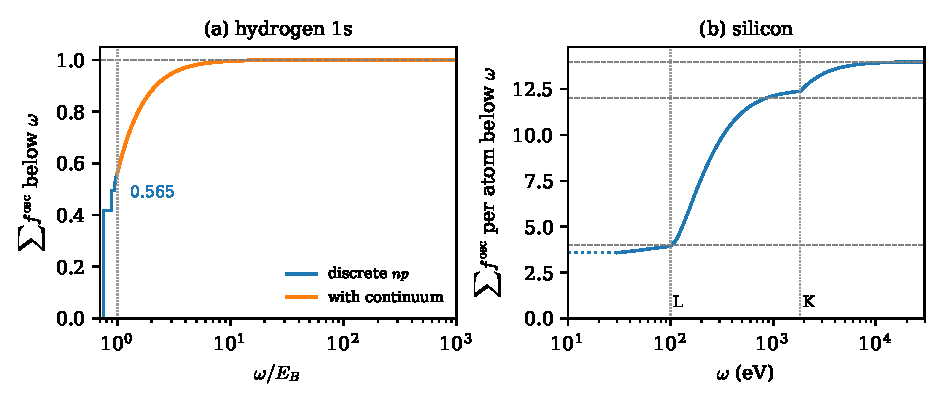
\includegraphics[width=\linewidth]{figures/ch04/fig4_3b.pdf}
  \caption{The Thomas--Reiche--Kuhn sum accumulated with energy. (a) Hydrogen in its ground state: oscillator strength of all transitions below the absorbed energy $\omega$, in units of the binding energy $E_B = \SI{13.6}{eV}$, from the closed forms of Bethe and Salpeter. The bound 1s--$np$ lines (steps, starting with 2p at $\tfrac34E_B$) carry 0.565 and the continuum 0.435; the total is one electron (dashed). (b) Silicon, per atom: oscillator strength below $\omega$ from the photoabsorption tables of Henke and coworkers above \SI{30}{eV}, integrated as $\dd f^{\mathrm{osc}}/\dd\omega = 2f_2/\pi\omega$, and offset so that the total, with the region above \SI{30}{keV} extrapolated as a power law, is 14. The offset, 3.58, is the strength below \SI{30}{eV} that the rule requires (dotted). Dashed lines mark 4 valence electrons, 4 + 8 and 14; dotted vertical lines the L and K edges at \SI{99.8}{eV} and \SI{1.839}{keV}.}
  \label{fig:4-trk}
\end{figure}
